% Model 2 conceptual schematic: (left) cohort decomposition & exact linearisation,
% (right) within-year timing of capital, water, upkeep and next-year PV revenue.
% Build: cd Paper/Figure && pdflatex m2_cohort_concept.tex
\documentclass[tikz,border=3pt]{standalone}
\usepackage{newtxtext,newtxmath}
\usepackage{amsmath,bm}
\usetikzlibrary{arrows.meta,decorations.pathreplacing,calc,backgrounds}
% Shared colours for the TikZ schematics; same roles and hex values as
% Code/figures_matlab/paper_style.m (mycolor.space, base #1E5F74).
%   water (P, I, M, W-bar)  teal   | vegetation (V, r, d)  green
%   wind and sand (E, S)    brown  | highlight             orange
%   limits and caps         red dashed
\definecolor{pWater}{HTML}{1E5F74}
\definecolor{pWaterMid}{HTML}{659FB6}
\definecolor{pWaterLight}{HTML}{DCEBF1}
\definecolor{pTeal}{HTML}{00828C}
\definecolor{pVeg}{HTML}{2B633C}
\definecolor{pVegMid}{HTML}{4AC087}
\definecolor{pVegLight}{HTML}{E3F3E8}
\definecolor{pSand}{HTML}{8F7159}
\definecolor{pSandLight}{HTML}{FFEACE}
\definecolor{pAccent}{HTML}{F49431}
\definecolor{pPV}{HTML}{D47216}
\definecolor{pPVLight}{HTML}{FDF1E3}
\definecolor{pPlum}{HTML}{7A437F}
\definecolor{pPlumLight}{HTML}{F2EBF3}
\definecolor{pLimit}{HTML}{D03B3B}
\definecolor{pInk}{HTML}{1F2B33}
\definecolor{pAxis}{HTML}{344A53}
\definecolor{pGrey}{HTML}{97AFB9}
\definecolor{pGreyDark}{HTML}{647B84}
\definecolor{pGrid}{HTML}{E6EBED}

\tikzset{
  badge/.style={circle, draw=#1, fill=white, line width=0.85pt, inner sep=0.6pt,
    font=\scriptsize\bfseries, text=#1, minimum size=11pt},
  flow/.style={-{Stealth[length=5pt,width=4pt]}, line width=0.85pt, draw=#1},
  track/.style={rounded corners=2pt, line width=0.75pt},
}
\begin{document}
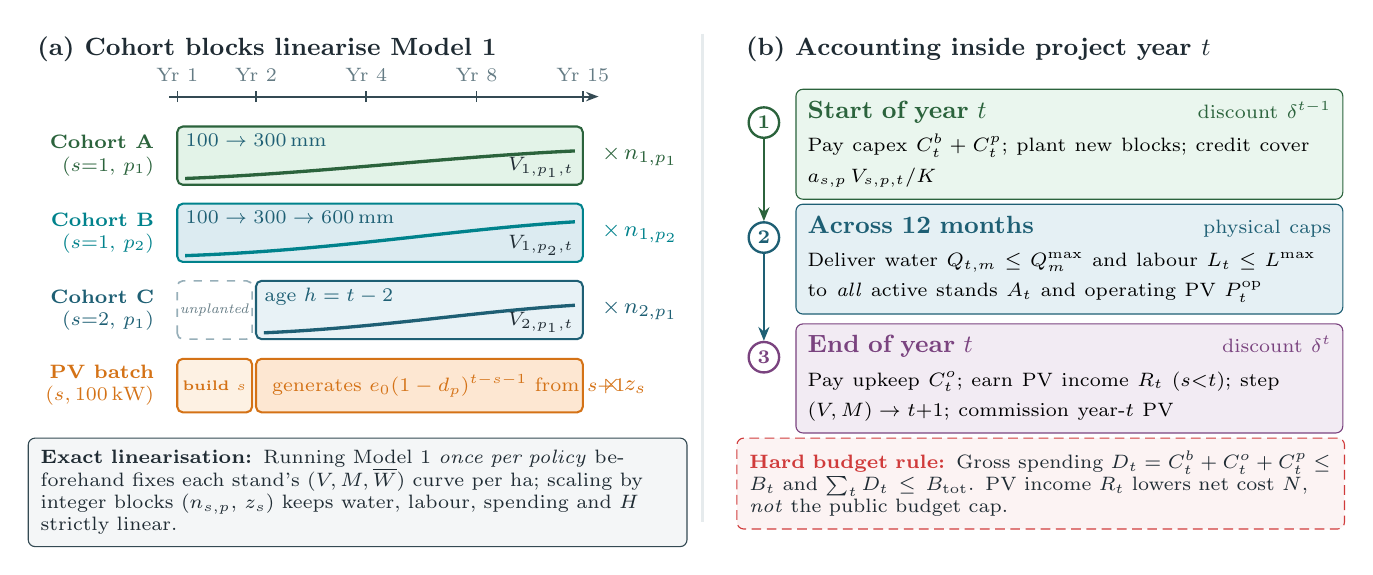
\begin{tikzpicture}[font=\small]

% ======================================================================
% LEFT PANEL: Cohort decomposition turns nonlinear Model 1 into linear sums
% ======================================================================
\node[font=\small\bfseries, text=pInk, anchor=west] at (0.05, 4.05)
  {(a) Cohort blocks linearise Model 1};

% Timeline header
\draw[-{Stealth[length=4.5pt]}, pAxis, line width=0.7pt] (1.85, 3.45) -- (7.30, 3.45);
\foreach \x/\lab in {1.95/Yr 1, 2.95/Yr 2, 4.35/Yr 4, 5.75/Yr 8, 7.10/Yr 15} {
  \draw[pAxis, line width=0.55pt] (\x, 3.38) -- (\x, 3.52);
  \node[font=\scriptsize, text=pGreyDark, anchor=south] at (\x, 3.52) {\lab};
}

% Cohort A (yr 1, step 100 -> 300)
\node[anchor=east, align=right, font=\scriptsize, text=pVeg] at (1.78, 2.70)
  {\textbf{Cohort A}\\$(s{=}1,\,p_1)$};
\fill[pVegLight, track, draw=pVeg] (1.95, 2.33) rectangle (7.10, 3.07);
\draw[pVeg, line width=1.2pt] (2.05,2.41) .. controls (3.8,2.48) and (5.3,2.68) .. (7.00,2.76);
\node[font=\scriptsize, text=pWater, anchor=north west, inner sep=2pt] at (1.98, 3.05) {$100\to 300$\,mm};
\node[font=\scriptsize, text=pInk, anchor=south east, inner sep=2pt] at (7.06, 2.34) {$V_{1,p_1,t}$};
\node[font=\footnotesize\bfseries, text=pVeg, anchor=west] at (7.22, 2.70) {$\times\,n_{1,p_1}$};

% Cohort B (yr 1, ramp 100 -> 300 -> 600)
\node[anchor=east, align=right, font=\scriptsize, text=pTeal] at (1.78, 1.72)
  {\textbf{Cohort B}\\$(s{=}1,\,p_2)$};
\fill[pWaterLight, track, draw=pTeal] (1.95, 1.35) rectangle (7.10, 2.09);
\draw[pTeal, line width=1.2pt] (2.05,1.43) .. controls (4.0,1.50) and (5.4,1.76) .. (7.00,1.86);
\node[font=\scriptsize, text=pWater, anchor=north west, inner sep=2pt] at (1.98, 2.07) {$100\to 300\to 600$\,mm};
\node[font=\scriptsize, text=pInk, anchor=south east, inner sep=2pt] at (7.06, 1.36) {$V_{1,p_2,t}$};
\node[font=\footnotesize\bfseries, text=pTeal, anchor=west] at (7.22, 1.72) {$\times\,n_{1,p_2}$};

% Cohort C (yr 2, shifted start!)
\node[anchor=east, align=right, font=\scriptsize, text=pWater] at (1.78, 0.74)
  {\textbf{Cohort C}\\$(s{=}2,\,p_1)$};
\draw[pGrey, dashed, line width=0.6pt, rounded corners=2pt] (1.95, 0.37) rectangle (2.90, 1.11);
\node[font=\tiny\itshape, text=pGreyDark] at (2.42, 0.74) {unplanted};
\fill[pWaterLight!65, track, draw=pWater] (2.95, 0.37) rectangle (7.10, 1.11);
\draw[pWater, line width=1.2pt] (3.05,0.45) .. controls (4.6,0.52) and (5.7,0.72) .. (7.00,0.80);
\node[font=\scriptsize, text=pWater, anchor=north west, inner sep=2pt] at (2.98, 1.09) {age $h=t-2$};
\node[font=\scriptsize, text=pInk, anchor=south east, inner sep=2pt] at (7.06, 0.38) {$V_{2,p_1,t}$};
\node[font=\footnotesize\bfseries, text=pWater, anchor=west] at (7.22, 0.74) {$\times\,n_{2,p_1}$};

% PV asset row (yr s, operates from s+1)
\node[anchor=east, align=right, font=\scriptsize, text=pPV] at (1.78, -0.22)
  {\textbf{PV batch}\\$(s,\text{100\,kW})$};
\fill[pPVLight, track, draw=pPV] (1.95, -0.56) rectangle (2.90, 0.12);
\node[font=\tiny\bfseries, text=pPV] at (2.42, -0.22) {build $s$};
\fill[pAccent!22, track, draw=pPV] (2.95, -0.56) rectangle (7.10, 0.12);
\node[font=\scriptsize, text=pPV, anchor=west] at (3.03, -0.22) {generates $e_0(1-d_p)^{t-s-1}$ from $s{+}1$};
\node[font=\footnotesize\bfseries, text=pPV, anchor=west] at (7.22, -0.22) {$\times\,z_s$};

% Key takeaway box under left panel
\node[draw=pAxis, fill=pGrid!45, rounded corners=2.5pt, text width=8.05cm, align=left,
      inner sep=4.5pt, font=\scriptsize, text=pInk, anchor=north west] at (0.05, -0.88)
  {\textbf{Exact linearisation:} Running Model~1 \emph{once per policy} beforehand fixes each stand's $(V,M,\overline W)$ curve per ha; scaling by integer blocks $(n_{s,p},\,z_s)$ keeps water, labour, spending and $H$ strictly linear.};

% ======================================================================
% RIGHT PANEL: Within-year accounting & commissioning clock
% ======================================================================
\begin{scope}[xshift=8.95cm]
\node[font=\small\bfseries, text=pInk, anchor=west] at (0.10, 4.05)
  {(b) Accounting inside project year $t$};

% Stage 1: Year start
\node[badge=pVeg] (b1) at (0.45, 3.12) {1};
\node[draw=pVeg, fill=pVegLight!75, rounded corners=2.5pt, text width=6.65cm, align=left,
      inner sep=4.2pt, anchor=north west] (st1) at (0.85, 3.55) {%
  {\color{pVeg}\textbf{Start of year $t$} \hfill {\scriptsize discount $\delta^{t-1}$}}\\[1pt]
  {\scriptsize Pay capex $C_t^b + C_t^p$; plant new blocks; credit cover $a_{s,p}\,V_{s,p,t}/K$}};

% Stage 2: Within year (12 months)
\node[badge=pWater] (b2) at (0.45, 1.66) {2};
\node[draw=pWater, fill=pWaterLight!75, rounded corners=2.5pt, text width=6.65cm, align=left,
      inner sep=4.2pt, anchor=north west] (st2) at (0.85, 2.09) {%
  {\color{pWater}\textbf{Across 12 months} \hfill {\scriptsize physical caps}}\\[1pt]
  {\scriptsize Deliver water $Q_{t,m}\le Q_m^{\max}$ and labour $L_t\le L^{\max}$ to \emph{all} active stands $A_t$ and operating PV $P_t^{\mathrm{op}}$}};

% Stage 3: Year end
\node[badge=pPlum] (b3) at (0.45, 0.14) {3};
\node[draw=pPlum, fill=pPlumLight, rounded corners=2.5pt, text width=6.65cm, align=left,
      inner sep=4.2pt, anchor=north west] (st3) at (0.85, 0.57) {%
  {\color{pPlum}\textbf{End of year $t$} \hfill {\scriptsize discount $\delta^{t}$}}\\[1pt]
  {\scriptsize Pay upkeep $C_t^o$; earn PV income $R_t$ ($s{<}t$); step $(V,M)\to t{+}1$; commission year-$t$ PV}};

\draw[flow=pVeg]   (b1.south) -- (b2.north);
\draw[flow=pWater] (b2.south) -- (b3.north);

% Hard budget limit callout at bottom right
\node[draw=pLimit, dash pattern=on 3.5pt off 2pt, fill=pLimit!6, rounded corners=2.5pt,
      text width=7.40cm, align=left, inner sep=4.5pt, font=\scriptsize, text=pInk, anchor=north west]
      at (0.10, -0.88)
  {{\color{pLimit}\textbf{Hard budget rule:}} Gross spending $D_t = C_t^b + C_t^o + C_t^p \le B_t$ and $\sum_t D_t \le B_{\mathrm{tot}}$. PV income $R_t$ lowers net cost $N$, \emph{not} the public budget cap.};
\end{scope}

% subtle divider between (a) and (b)
\draw[pGrid, line width=0.9pt] (8.62, 4.25) -- (8.62, -1.95);

\end{tikzpicture}
\end{document}
